\chapter{乘法}

\section{乘法的起源}
人们使用乘法已经有数千年的历史。乘法是在解决各种实际问题的过程中逐渐发展起来的。让我们从某个具体的实际问题出发,看看乘法到底是什么``法"?

如图\ref{img_multiplication},我们可以想象一片空地,现在的任务是用同样大小的方砖把阴影部分铺满,那么一共需要多少块砖呢?我们可以从离我们最近的地方,从左到右铺满一行, 恰好发现需要4块方砖就够了,所以我们先记下每行4块。然后,我们在最左边从下到上接着铺,发现只需3块方砖就可以铺到上边的边界,于是我们知道一共需要3行。 虽然我们还没有铺满阴影部分,但我们已经知道我们需要\textbf{每行4块 一共3行}。

\begin{figure}[h]
    \center
    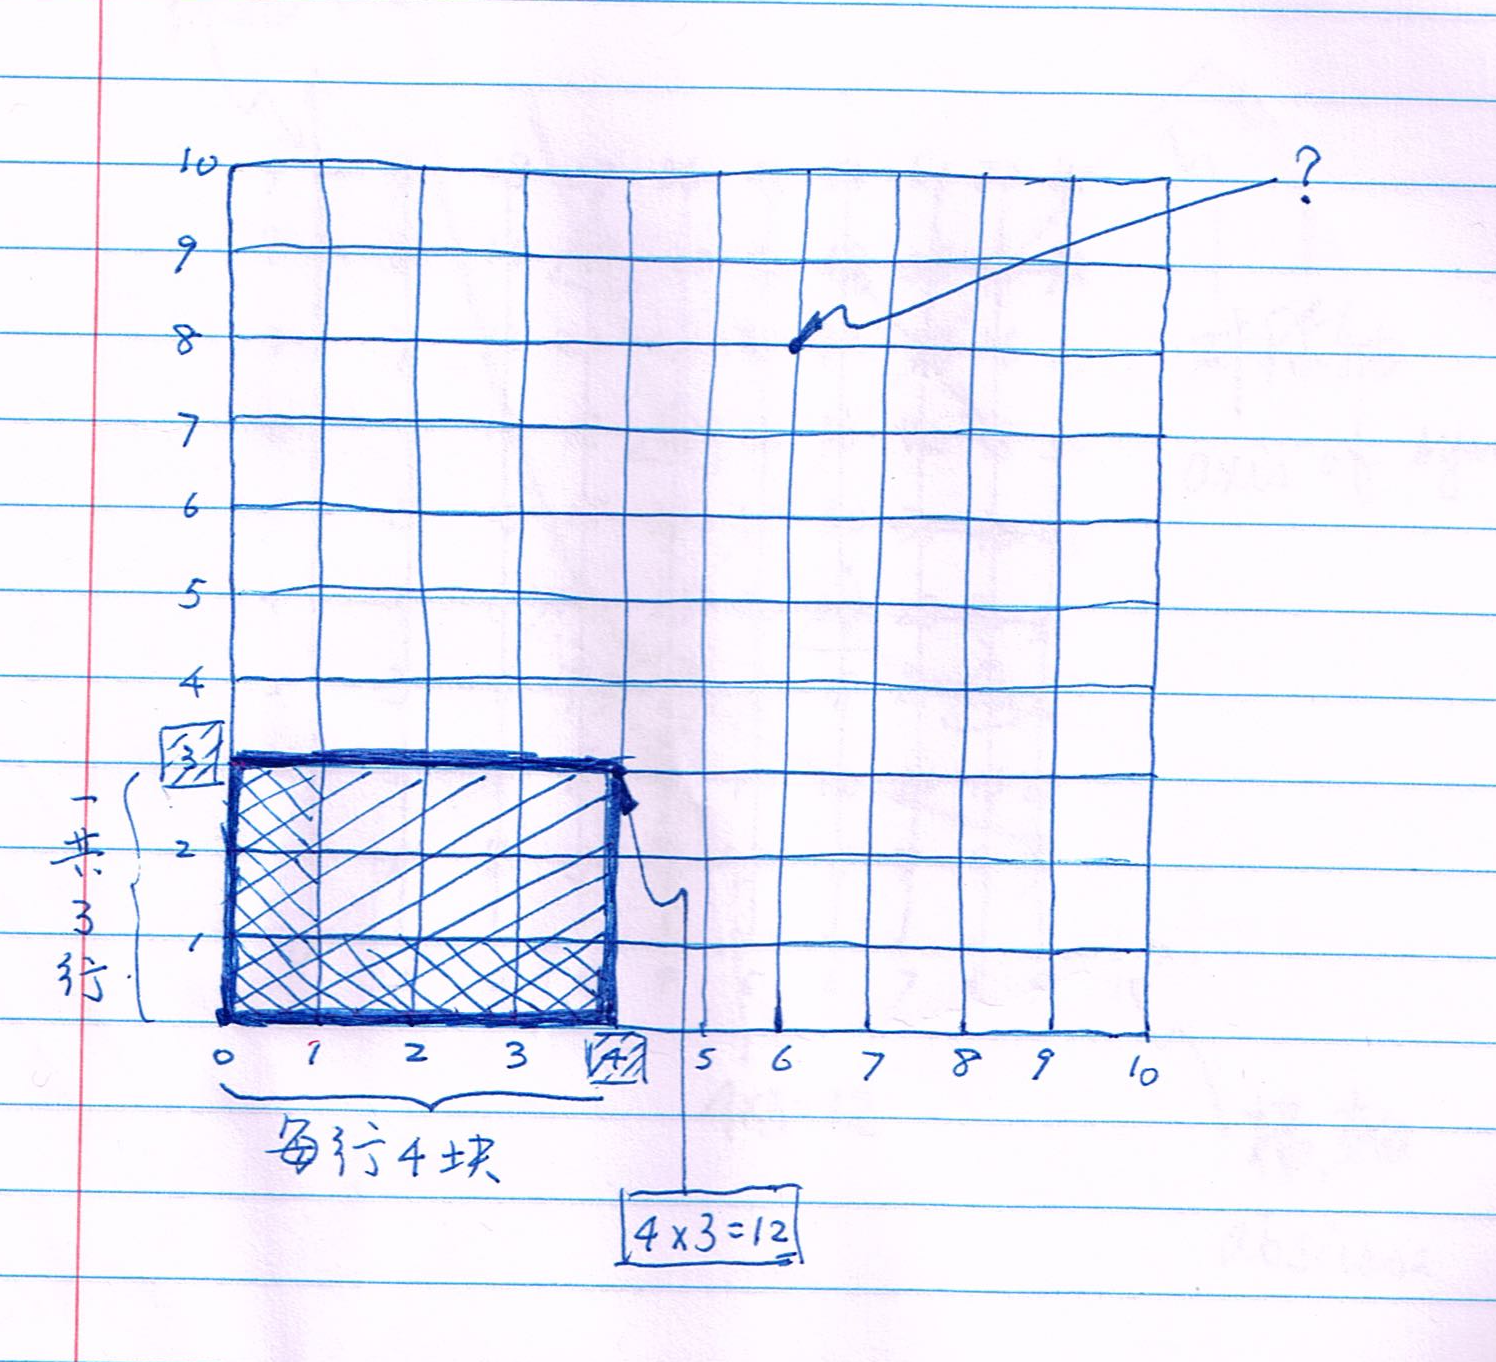
\includegraphics[width=0.8\textwidth]{multiplication_res/multiplication_definition}\label{img_multiplication}
    \caption{乘法的定义。}
\end{figure}


如果我们想要铺满另一块地,用同样的方法,我们可能会发现类似的结果,但是具体数字可以有所不同,比如
\begin{itemize}
    \item 每行6块
    \item 一共8行
\end{itemize}
我们只要知道两个数:(1)每行需要几块砖,(2)一共需要几行,就可以知道总共需要多少砖来铺满某块地。为了方便记录,我们用乘号$\times$来连接这两个数字。

上面提到的第一种情况就可以记录成$4\times3$,而第二种情况可以记录成$6\times8$。

这就是乘法的应用场景之一。有时人们就把阴影部分叫做$4\times3$ (four by three) 的区域,把第二种情况叫做$6\times8$的区域。

\section{乘法与加法}
现在,我们还没有回答到底需要多少块砖才能铺满图中的阴影部分。也就是说我们要计算$4\times3$等于多少。如果我们把阴影部分铺满,完成第一行时用了4块砖,

完成第二行又用了4块砖,完成第三行接着用了4块砖,这样一共需要$4 + 4 + 4 = 12$块砖。这种计算方法告诉我们$4\times3 = 4 + 4 + 4$也就是说$4\times 3 = 12$。

那么对于第二种情况,$6\times 8 = 6 + 6 + 6 + 6 + 6 + 6 + 6 + 6$, 也就是说 $6\times 8 = 48$。

很显然,如果用加法,我们需要铺满整个阴影部分才能知道结果,如果使用乘法,只需要铺满最下面和最左边的边界就可以了。这就节省了很多重复性的记录。

对于刚才的两个例子来说,特别是第二种情况下使用乘法,是不是更加简洁?如果需要18行砖,每行26块,用乘法记录,也只需要两个数($26\times 18$)。如果用加法呢?换句话说,对于这类问题,乘法具有可扩展性(scalable)。当然,乘法的结果还是要通过加法来计算,不过,由于乘法可以用到很多地方,

人们总结了一个乘法表,可以直接查到乘法的结果,不需要每次都使用加法来计算了。
\subsection{乘法表的使用} 图\ref{img_multiplication_table}就是乘法表,它和图\ref{img_multiplication}一样,不过在每一个点上都记录了一个乘法计算的结果。比如,我们刚才想知道$4\times3$,就可以先从横轴上找到4,然后向上走3步,
也就是纵轴上的3一样高的时候,这个点上的数值12就是$4\times3$的结果,称作积(product)。或者,可以右手食指先沿着横轴找到4,左手食指沿着纵轴找到3,

然后右手向上走,左手同时向右走,两只手食指会和的地方就是12,也就是4 X 3 = 12。下面,大家可以找一下6 X 8等于多少?大家试一试,如果只用一只手指,能够使用乘法表么?

\begin{figure}[h]
\center
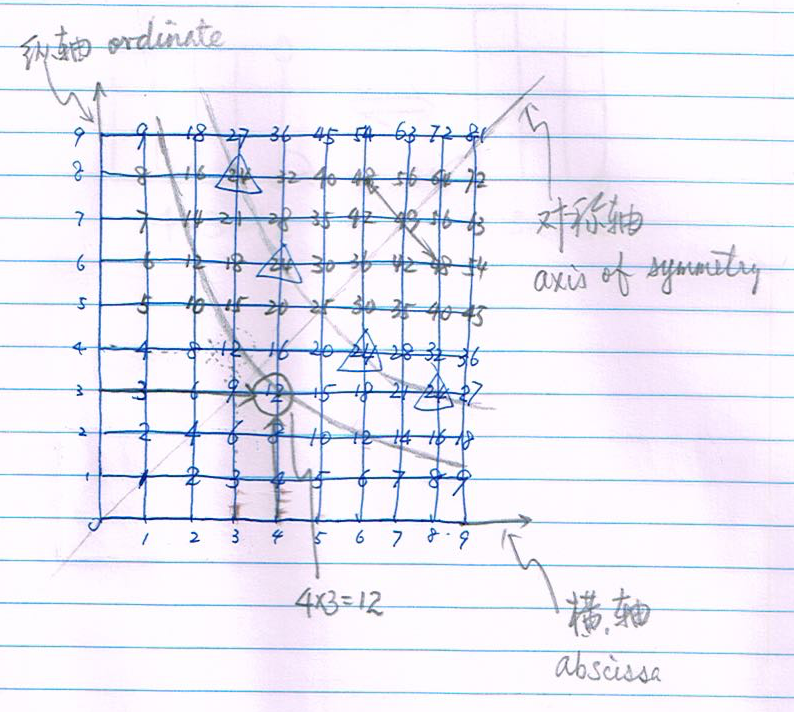
\includegraphics[width=0.8\textwidth]{multiplication_res/multiplication_table}\label{img_multiplication_table}
\caption{乘法表}
\end{figure}

如果大家记住了乘法表,可以很快的计算出乘法的结果。当你把乘法表背得滚瓜烂熟,就可以用它解决更加有趣的问题。
\subsection{乘法表的有趣之处}
\subsubsection{1的特殊之处}
利用乘法表,计算5X1,6X1,7X1,有什么规律么?

\subsubsection{对称轴与交换律}
刚才我们用乘法表算出了$4\times3=12$。大家找一找,这个表里面还有没有12?有一个12是用虚线圈起来的。想一想,计算什么的时候我们才会找到那个虚线圈起来的12呢?答案是$3\times4$。
刚才我们还算出了$6\times8 = 48$,那么$8\times6$ 是多少?

这就是说,乘法具备交换律 (commutative)。如果把乘号两边的数字交换一下,结果是相同的。

在这个图上,还画了一条对称轴(axis of symmetry) ,刚才找到的两个12,和两个48,都在这个对称轴的两边,并且和这条对称轴的距离一样。这时我们就说他们关于这条轴是对称的。大家再看看,是不是距离对称轴同样距离的数字都是一样的?如果这样,那么我们还需要整张乘法表么?

实际上,大部分的乘法表都只有上半部分,或是下半部分?如果只有下半部分,我们还可以找到$6\times8$么?不能了吧?但是别忘了我们还有交换律。

\emph{交换律的几何解释}

为什么乘法会有交换律呢?我们回想一下4X3 的来源。最初,我们希望计算图一	中阴影部分需要多少块砖,发现需要每行4块砖,一共摆3行(4 X 3)。

如果我们把这块地转一下(图\ref{img_commutative}),所需砖的数目是不变的,但是这样就变成每行3块转,一共需4行(3 X 4)。既然这两种情况所需方砖数目一样,4X3当然要等于 3 X 4了。

一块空地当然是转不动的,但是我们上面的解释大家都可以接受,这就是所谓思想实验(thought experiment)。思想实验是数学家,哲学家和理论物理学家的常用工具。

\begin{figure}[h]
    \center
     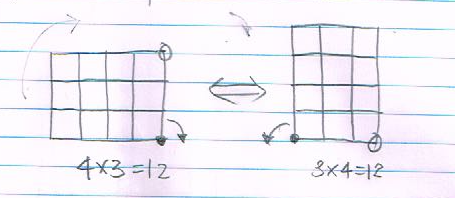
\includegraphics[width=0.4\textwidth]{multiplication_res/commutative}
     \caption{交换律的几何几何解释。}
     \label{img_commutative}
\end{figure}

\emph{双曲线}

乘法表里(图\ref{img_multiplication_table})一共有几个地方有12呢?我们还能找到$6\times2 = 12$和 $2\times6 = 12$。如果还用铺砖作为例子,$6\times2$ 的意义是什么呢?它铺的是哪一部分呢?

试着自己画一下。现在我们知道, $6\times2 = 4\times3 = 3\times4 = 2\times 6$。回忆一下,第一个数字表示每行需要几块砖,第二个数字表示一共需要几行,如果每行需要的砖更多,需要的行数是更少还是更多呢?如果需要的行数更多,每行的砖数是更多还是更少?

我们把这样的关系称作反比。如果所需方砖总数一定,每行的砖数和所需行数成反比。换句话说,如果我和你各自有12块方砖,如果我铺的比你宽,你肯定铺的行数比我多。不可能我铺的比你宽,而且行数也比你多。实际生活中那个,我们往往会遇到这样的情况,由于具体条件的制约,我们必须在互成反比的东西中间作出取舍,选择更加重要的东西。这就是成语里说的鱼与熊掌不可得兼。
 
 试着把所有等于12的点连起来,再试着把所有等于24的点连起来,这样的线叫双曲线(hyperbola)。这些双曲线会不会相交呢?为什么不会?还用铺砖的例子解释一下。(反证法)
 
想象一下你在双曲线的某个点(三角形标注的点)上,写下对应的乘法表达式,和对应的方砖所铺满的地域,当你向下滑倒另一个点时, 写下对应的乘法表达式和对应的地域,体会宽度的行数的变化关系。

\subsection{乘法的应用}
\subsubsection{面积与平方}
人们通常关心一块地方的大小。还是以铺砖为例,大的地方需要更多的砖,因此,砖的数目就可以让人们方便的记录和比较地方的大小。地的大小又叫做面积(area)。图一里阴影部分的面积就是12。前面也讨论过,有几种不同的铺砖方法可以覆盖同样大小的面积。

你可能注意到,如果我们用的方砖大小不一样,即使都用12块砖,他们的面积也是不一样的。所以,为了准确的描述总面积,我们还需要知道所用方砖的面积。比如,方砖的边长可以是1米,它的面积就称作1平方米。12块砖的总面积就是12平方米。

如果每块方砖的边长是2米呢?这种大方砖相当于两行刚才用的小方砖,并且每行有两个,这样的大方砖相当于$2\times2 = 4$ 个小方砖,因为小方砖的面积是1平方米,大方砖的面积就是4平方米(不是2平方米)。

乘法表的对称轴上,是两个相同的数字的积。比如$5\times5 = 25$。两个相同数字相乘,又叫做平方(square)。再回忆一下铺砖的例子,$5\times5$的意思是每行有5块方砖,共需5行,总共要5的平方也就是25块砖。试着画一下这块地方,是不是一个正方形(square)?如果用前面的小方砖,面积就是25平方米。如果用大方砖呢?每行需要10块小方砖,共需10行,也就是说需要$10\times10=100$块小方砖,总面积100平方米。换一个办法,我们已经知道大方砖的面积是4平方米,一共需要25块大方砖,那么总面积是多少呢?$4+4+4+...+4$?我们前面是不是遇到过这种连加的问题,最然这次不是多少行砖的问题,但是数学式子是类似的,可以用乘法表示么?

再回到图一的阴影面积。我们用边长1米的方砖,如果每行需要4个,也就是说阴影部分的宽是4米,如果共需3行,也就是说阴影部分的高是3米。前面算过,它的面积是$4\times3$,也就是长$\times$宽。

\subsubsection{连乘、立方与体积}

乘法当然并不局限于两个数。如果我们需要在图一的阴影部分铺5层砖,那么一共需要多少块呢?$4\times3 + 4\times3 + 4\times3 + 4\times3 + 4\times3$ 如果用乘法,是不是可以简化成$(4\times3)\times5$。注意,这里的括号表示我们要先计算$4\times3$,再用等到的结果12和5相称。你能在乘法表上找到$12\times5$的答案么?

刚才讨论过乘法交换律,并且用图\ref{img_commutative}的旋转法做了解释。乘法还满足结合律(associative)。 也就是说,$(4\times3)\times5 = 4\times(3\times5)$。你能试着用类似的方法解释么?


比较一块地的大小可以用面积,这里,我们又引入了砖的层数,这一堆砖所占空间的大小称为体积(volume)。体积可以用每层面积$\times$层数来计算。面积和体积,都用到了积这个字,也都用乘法计算,现在可以理解,为什么用积来称呼乘法的结果了吧。面积和体积,差别就在于一个用来描述平面的大小,另一个用来描述物体的大小。如果四个数连乘,有什么意义么?等你上了大学,就可以学到高维空间,那里面的体积就要4个数,甚至成千上百个数连乘来计算体积。

和刚才一样,一堆砖的体积不仅和方砖的数目有关,还和方砖的大小有关。如果方砖的长、宽、高均为1米,每块的体积称为1立方米,上面的两层砖总体积为$4\times3\times5$立方米。如果使用长宽高均为2米的大方砖,每块的体积是多少呢?

\subsubsection{糖果的数量}
    
乘法还有别的应用。比如,如果一包糖果里有10颗糖,一共有3包,那么一共有几颗糖?

    $10 + 10 + 10$
  
我们前面用乘法解决过这个问题,也就是$10X3=30$。

如果我们还有3颗散装的糖果,一共有几颗呢?

    $(10\times3) + 3 = 33$

 我们约定,乘法要最先计算,所以,这里的括号也可以省略?你知道为什么乘法要先计算么?(见下一条)

 如何计算下面的糖果数量:
 \begin{itemize}
    \item 5整包,2散装:$10\times5+2$
    \item 8整包,7散装:$10\times8+7$
    \item 2整包,4散装:$10\times2+4$
 \end{itemize}
 

\subsubsection{位的概念}
刚才记录糖果总数的时候,其实只需要记录有多少包整的,和多少散装的,
\begin{itemize}
 \item 5整包,2散装:$10\times5+2 = 52$
 \item 8整包,7散装: $10\times8+7 = 87$
 \item 2整包,4散装:$10\times2+4 = 24$
\end{itemize}

这里,我们约定,第一个数字记录有多少包,第二个数字记录有多少散装的。而且,我们约定,每包必须有10颗糖。这种计数方式称为十进制。

它第一个数字称作十位,第二个数字称作个位。十位上的数字代表整包的数量,每增加1,相当于增加了一包,也就是10颗糖。个位数字代表散装的数目,它只可以是0到9。如果现在有29颗糖,再加上一颗之后,就可以凑成3整包,也就是30颗糖。

如果糖的数目是64,怎么用乘法和加法表示呢?$64=10\times6+4$。如果先计算加法,再计算乘法,
    $64=10X6+4
        =10X(6+4)  这样先算加法是错误的
        =10X10$  这就不是64了。
    
 这就是为什么大家约定要先计算乘法,再计算加法。

 为什么大家使用十进制呢?有一种说法是,古人用手指计数,如果数字大于10,比如13,就用一个脚趾记录10,三个手指记录3。如果63,需要几个脚趾和几个手指呢?用这种方法最多能记录多大的数字呢?

 如果有个星球上的外星人有8个手指和8个脚趾,他们会发明什么计数方式呢?是不是叫做八进制?他们的63相当于地球上的多少呢?他们所能记录的最大数字是多少呢?

  十位上增加1,相当于增加了10个,这就是成语所说的以一当十。如果,数字继续增加,我们就需要更高的位数,比如百位、千位。百位的增加1,相当于十位增加了10个,也就是增加了10个10,我们把它叫做一百(100)。所谓十进制,就是计数到10就要进到上一位。相邻两位之间存在以一当十的关系。
    \begin{eqnarray}
    235 &=& 10\times10\times2 + 10\times3 + 5, \\
    1235 &=& 10\times10\times10\times1 + 10\times10\times2 + 10\times3 + 5
    \end{eqnarray}
  再思考一下,如果用糖果做例子,交换律该如何解释呢。

\subsubsection{分配律}

如果在铺满了图\ref{img_multiplication}的阴影部分后,我们又需要铺第二块区域(图\ref{img_distributive})。按照前面的记法,	第二块区域每行需要2块方砖,一共需要3行。或者说,这是$2\times3$的区域。一共需要的方砖数是
$4\times3+2\times3$。

\begin{figure}[h]
    \center
    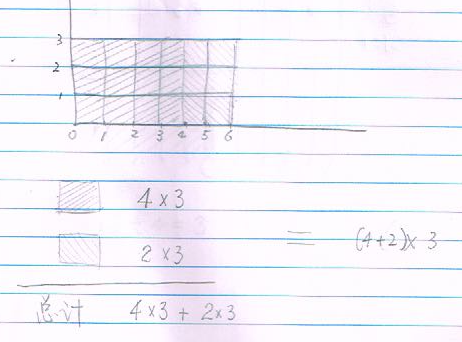
\includegraphics[width=0.4\textwidth]{multiplication_res/distributive} 
    \caption{}
    \label{img_distributive}
\end{figure}

  如果我们一开始就知道要铺满整块区域,那么每行需要6块方砖,一共需要3行。或者	说这是$6\times3$的区域。一共需要的方砖数是
    $6\times3 = 18$。(你还需要看乘法表么?)

  不管是分两次铺,还是一次铺完,方砖的总数是一样的,也就是说,
  \begin{eqnarray}
    4\times3+2\times3 &=& 6\times3,\\
    4\times3+2\times3 &=& (4+2)\times3
  \end{eqnarray}
  
  换句话说,我们可以把左边两项的共同点(X3)拿出来,先做4+2,然后把结果再乘以3。这个操作叫做提取公因子(把公共的因子3提取出来的意思)。之所以这样做,是因为乘法满足分配律(distributive)。

  提取公因子的好处是什么呢?我们看看这两种计算方法需要多少次乘法和多少次加法。
\begin{table}
    \center
    \begin{tabular}{c c c}
  &乘法的次数&加法的次数\\
\hline
    $4\times3+2\times3$&	2&	1\\
    $(4+2)\times3$&	1&	1
    \end{tabular}
\end{table}
    
  提取公因子之后,我们少用了一次乘法。也许在这个例子里,少用一次乘法并不是显著的改进。但是,如果我们要计算$4\times3+2\times3+5\times3+7\times3+9\times3$,如果直接计算,需要4次加法	和5次乘法,如果提取公因子,需要4次加法和1次乘法。如果有更多项相加,如果可	以提取公因子,乘法计算的次数还是1次。这是可扩展性的又一个例子。

  有时,我们还要把提取公因子的过程反过来。前面问到$12\times5$能不能从乘法表上查到。	答案是否定的。古人为什么没有把$12\times5$放到乘法表上呢?
  
  我们先想一想12X5怎么计算。因为乘法表上没有12,所以我们要把12用乘法表上包括的数字表示,比如
   $12\times5 = (8+4)\times5
    = 8\times5+4\times5$

  这样,乘法分配律可以帮助我们把一个表中没有的问题,化解成两个更加简单的问题。这个策略通常叫做分治(divide and conquer)。我们想一想,还有什么别的算法么?

  $12\times5 = (4\times3)\times5 = 4\times(3\times5)=3\times(4\times5)$? 这样做有帮助么?

  $12\times5=(10\times1+ 2)\times5
  = 10\times(1\times5) + 2\times5$

  这种方法认识到了十位的意义,用分配律之后,第一项$10\times(1\times5)$是不是意味着在十位上可以直接写上1X5的结果?这就是说,我们可以先用十位上的数字和5相乘,把结果放在十位上,然后再把个位上的数字和5相乘,最后把结果和第一步的结果相加。因为个位或者十位上最大的数就是9,所以我们的乘法表是够用的。回想一下只有八个手指的外星人,他们的乘法表中最大的乘数是多少呢?    

  理解了这种计算方法之后,要通过大量的练习,成为一种本能的反应。我们再举一个例子。
  \begin{eqnarray}
  32\times4 &=& (10\times3 + 2)\times4,\\
  &=& 10\times(3\times4) + 2\times4,\\
  &=& 120 + 8 ,\\
  &=& 128
  \end{eqnarray}

  第一步:10位的3和4相乘,结果是12。你能在十位上写两个数么?是不是1很自然	的站到了百位上。12个10,就是10个10加2个10,也就是120。

  第二步,个位的2和4相乘,结果是8。

  第三步,把前两步的结果加起来。

  你能试着算算12X13么?

  为了方便计算,古人发明了竖式(图\ref{img_shushi})。你能用学到的分配律解释这种算法么?
  
  \begin{figure}[h]
       \center
       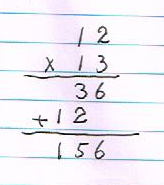
\includegraphics[width=0.3\textwidth]{multiplication_res/shushi}
       \caption{竖式}
       \label{img_shushi}
  \end{figure}
\subsection{十进制的历史}
中国人使用十进制和乘法表已经有超过三千年的历史。有的古文明不采用十进制。比如	古巴比伦人采用60进制,他们的乘法表需要多大呢?

考古发现,巴比伦人的乘法表里	只有平方。也就是说,你只能查到$1\times1=1,2\times2=4,3\times3=9,...,59\times59=3481$。那么巴比伦人如何计算$12\times5$呢?

试试分治法?

$12\times5=(6\times2)\times5 = 6\times10 = (8-2)\times(8+2) = (8-2)\times8 + (8-2)\times2 = 8\times8-2\times8+8\times2-2\times2  = 64 - 4 = 60$


